\documentclass{article}
\usepackage{color}
\usepackage{placeins}
\usepackage{listings}
\usepackage{graphicx}
\usepackage{xcolor}
\usepackage{amsmath}
\usepackage{subcaption}
\usepackage{cleveref}
\usepackage{booktabs}
\usepackage{geometry}[margins=1in]
\setlength{\parskip}{4pt plus 2pt}
\setlength{\parindent}{0pt}
%\pagecolor[rgb]{0,0,0} %black
%\color[rgb]{1,1,1} %grey
\lstset{language=C++,
keywordstyle=\color{blue},
stringstyle=\color{red},
commentstyle=\color{green},
morecomment=[l][\color{magenta}]{\#},
breaklines=true,
breakatwhitespace=true,
numbers=left
}

\usepackage{siunitx}

\title{Assignment \#3}
\author{Asbjørn Bonefeld Preuss,\\ Daniel Lomholt Christensen,\\ Elie Cueto}
\date{February 2024}
\setlength{\textheight}{1.05\textheight}
\begin{document}
\maketitle
\pagenumbering{roman}
\renewcommand{\thesection}{Task \arabic{section}:}
\renewcommand{\thesubsection}{Subtask \arabic{section}\Alph{subsection}:}
\newpage
\pagenumbering{arabic}
\section{Write a functioning master-worker program}
A simple program was written which implements a master worker program using OpenMPI. This code can be seen in section \ref{sec: task farm source}. Our master routine is defined on lines $36$--$87$, and the worker routine is defined on lines $108$--$127$. 

The master in this program makes a list of the tasks that are currently being processed by workers. This list is then initially filled, as tasks are sent out to all workers available.

The following loop then runs until all tasks are done.
As a worker finishes a \verb|task_function|, the master receives a message back from that worker. The master then gets their rank and records it in a result array, and gives the worker a new task to perform.

After all these tasks are done, the master shuts down the workers by giving them a task value of -1.

The worker therefore just receives a message, performs its task, and sends it back, until it receives a message with the task value of -1.

Only blocking messages are used in this implementation of a simple master-worker program.

\section{Master-worker program for HEP data processing} 
The high energy physics code was restructured to allow for running the data reduction on multiple cores. The ideas and code from above were reused, with renaming of several variables, and other small changes, that integrated the previous solution into the HEP code. The code can be seen in section \ref{sec: task farm hep source}. Our master routine is defined on lines $153$--$209$, and the worker routine is defined on lines $249$--$272$. 

Importantly, the worker no longer sends its rank to the master. This is instead extracted from the \verb?MPI_Status? through \verb|status.MPI_SOURCE|.

\section{Strong scaling of HEP processing using SLURM}
\begin{figure}
\begin{subfigure}[t]{0.5\textwidth}
    \centering
    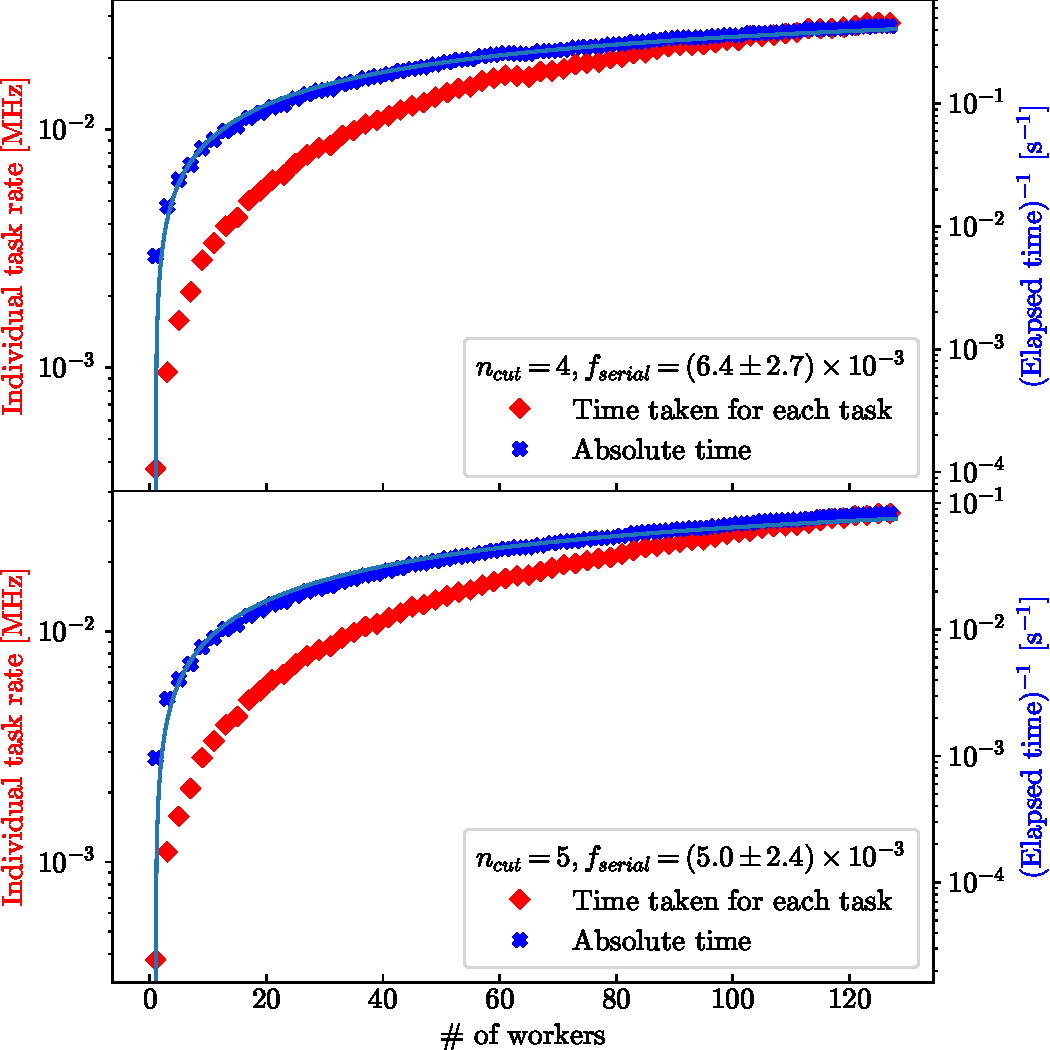
\includegraphics[width=\textwidth]{Assignment_3_Task_farming/Report/Amdahl.pdf}
    \caption{Strong scaling plots for $n_{cut}=4$ and $n_{cut}=5$, including fits to Amdahl's law}
    \label{fig:Amdahl}
\end{subfigure}
\begin{subfigure}[t]{0.5\textwidth}
    \centering
    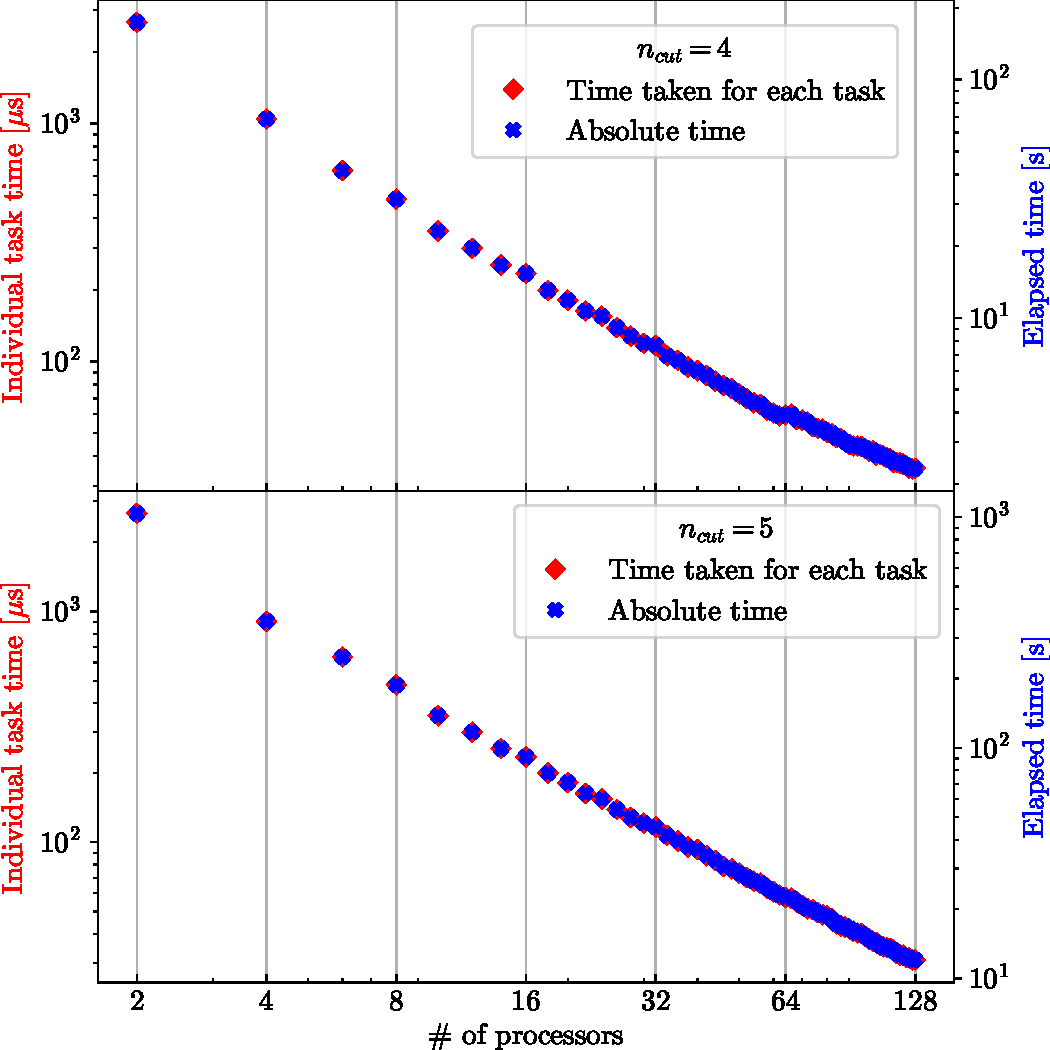
\includegraphics[width=\textwidth]{Assignment_3_Task_farming/Report/Time_scaling.pdf}
    \caption{Total run time and time per task as functions of number of processors for $n_{cut}=4$ and $n_{cut}=5$}
    \label{fig:Time}
\end{subfigure}
\caption{}
\end{figure}



\subsection{Experimental results}
In Fig. \ref{fig:Time} we show the total wall time and time per task for different numbers of processors between $2$ and $128$, and for $n_{cut}=4$ and $5$. In both of the plots and for both the total time and time per task, we see that the time decrease stalls slightly at $n_p=32$ and $64$, where the program starts having to communicate with respectively the other half of its own node, or another node entirely, so the latency increases with some of the CPUs, and the amount of speedup decreases.

In Fig. \ref{fig:CPU} we show the time spent per task per worker CPU core, for the same amounts of processors and values of $n_{cut}$ as above. In a perfect world the points here should all lie on a straight line. We see however, that this is not the case. Instead the value increases significantly at low numbers of processors, and then more slowly towards higher numbers. 

The low values for the lowest numbers of processors are found where the master only has to communicate with its immediate neighbours in the same NUMA die, and the subsequent increase up to around 32 cores are from the increased latency caused by having to communicate with cores in different NUMA dice. 

Above 32 processors the curve flattens out and increases slowly but linearly up to 64, as the latency in having to communicate with cores in the other 4 NUMA dice within the same node is about the same for each of the next 32 added cores. 

There is another jump in individual task time at 64 cores, when having to start talking to another node entirely. Above 64 cores the increase per added node is again about constant. Above 64 cores we also start seeing a significant difference between the $n_{cut}=4$ and $n_{cut}=5$ cases as well, with the $n_{cut}=4$ cases slowing down more quickly. %\textcolor{red}{\textbf{[I don't have a great explanation for why this is.]}}

We don't know exactly why this might be, but 
%that is beyond the scope of this assignment, and our guesses can be given upon inquiry.
our best guess is, that we get a greater use of the many workers, if we have enough tasks for all of them. In the case of $n_{cut}=4$, the fastest workers might be done with all of the available tasks before the slowest are done with their first. If this is the case, one could try implementing a feature, where idle worker-cores, get assigned the same task as someone else, and then whoever finishes first, gets to deliver a result. Another possibility is to simply cut the work into smaller bites.

\subsection{Serial and parallel fraction of the code}
In Fig. \ref{fig:Amdahl} we show the inverse wall time and inverse time per task for the same cases described above. These figures are proportional to the speedup gained over the serial run time. Therefore, we can estimate the parallel and serial fractions using Amdahl's Law:
\begin{equation}
    S = \frac{1}{(1-p)+\frac{p}{N}}
\end{equation}
where $S$ is the speedup factor, $p$ is the parallel fraction, and $N$ is the number of worker cores. Using this law we estimate the parallel and serial fractions for the $n_{cut}=4$ and $5$ cases respectively to be $p_4=0.994\pm0.003$,\; $s_4=0.006\pm0.003$,\; $p_5=0.995\pm0.002$, and $s_5=0.005\pm0.002$. The theoretical strong%weak 
scaling curves for these fractions are also shown in Fig. \ref{fig:Amdahl}, and we see that they line up rather well with the data. 

With these values of the serial fraction we expect the maximum possible theoretical speedup to be $S_{max,4}=167$ and $S_{max,5}=200$, in the case of an infinite number of cores. We have serial wall times of $T_{s,4}=\qty{173.5}{s}$ and $T_{s,5}=\qty{1033}{s}$, giving us speedup factors for the maximum tested number of cores of $S_4(128)=74.4$ and $S_5(128)=85.6$. These are very significant speedups, both around half of the maximum theoretical speedups.
\begin{figure}
    \centering
    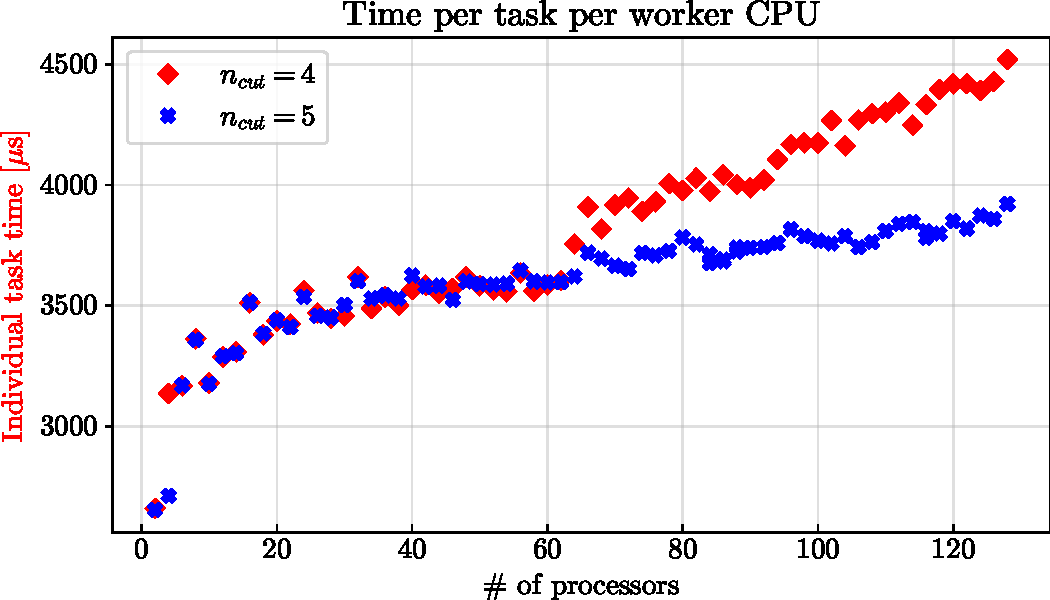
\includegraphics[width=1\textwidth]{Assignment_3_Task_farming/Report/CPU_time.pdf}
    \caption{Time per task per worker as functions of number of processors for $n_{cut}=4$ and $n_{cut}=5$}
    \label{fig:CPU}
\end{figure}
\subsection{The results in the context of strong scaling}
%It is difficult to test the strong scaling of this particular problem due to the way the size of the number of tasks to be performed scales as $n_{cut}^8$. That said, there is about a factor of $6$ difference between the number of tasks in the $n_{cut}=4$ and $5$ cases, so we can compare the $n_{cut}=5,n_{worker}=127$ to the $n_{cut}=4,n_{worker}=21$ cases, the $n_{cut}=5,n_{worker}=63$ to the $n_{cut}=4,n_{worker}=11$ cases, and the $n_{cut}=5,n_{worker}=31$ to the $n_{cut}=4,n_{worker}=5$ cases. These comparisons have been made in table \ref{tab:strong_scaling}, where we see a fairly constant speedup of a factor of $\sim 5$ when increasing the size of the problem by a factor of $\sim 6$. We cannot reasonably do this up to much higher values of $n_{cut}$ due to the way the size of the problem scales, but we do see a significant strong scaling speedup for the case we can test. 
%
%One caveat to this is that the best obtained accuracy for $n_{cut}=4$ and $5$ respectively are $0.73674$ and $0.73677$. This means that for a similar computation time, a six-fold increase in computational resources yields a $0.004\%$ improvement in results (if it is correctly understood that the goal is to find the best possible accuracy). Therefore is would seem that using a large number of CPU cores makes good sense for speeding up computations, but one should take into considerations how well results are actually improved when increasing the size of the problem. In this specific case there are most likely much faster ways of determining the best parameter values to maximize the accuracy, possibly even in serial, but in other problems this may not be the case in the same way.
%\begin{table}[]
%    \centering
%    \begin{tabular}{l|cc|cc|cc}
%         $n_{cut}$&5&4&5&4&5&4  \\
%         $n_{workers}$&127&21&63&11&31&5\\\midrule
%         Time [s]&12.1&10.7&22.5&19.6&45.4&41.5\\
%         Speedup &5.2&&5.2&&5.4\\        
%    \end{tabular}
%    \caption{Strong Scaling Comparisons between the $n_{cut}=4$ and $n_{cut}=5$ cases \textcolor{red}{\textbf{[Maybe this could do with some formatting]}}}
%    \label{tab:strong_scaling}
%\end{table}
From the fits, we see that the scaling of this problem is almost a text book example of Amdahl's law, often associated with strong scaling. In that case the speed-up will never be great. The high-energy physicists, needing to run this code, will be three quarters of the way to optimal speed\footnote{Given this code.} with just 600 workers, as opposed to infinite resources. If they want to gain another 25 in the speedup (total speed-up being 175), they would need around 1400 worker-cores. Since these extra computers aren't free, they  should definitely have a look at more effective algorithm first.
\newpage
\section{Task farm}
\label{sec: task farm source}
\lstinputlisting[language=c++]{../Code/task_farm.cpp}

\section{HEP Task farm}
\label{sec: task farm hep source}
\lstinputlisting[language=c++]{../Code/task_farm_HEP.cpp}

\end{document}
